% ***************************************************************************************************
%
%	Szablon pracy magisterskiej dla Politechniki Wrocławskiej w wersji dwustronnej.
%	Autor:	Tomasz Strzałka
%
% ***************************************************************************************************

% Styl dwustronny z domyślną wielkością czcionki 10pt oraz oddzieloną stroną tytułową (titlepage).
% Domyślnie rodziały rozpoczynają się na stronie prawej (openright).
\documentclass{book}

% ***************************************************************************************************
% Ustawienia języka
% ***************************************************************************************************

% Podstawowe ustawienia języka, według którego formatowany będzie dokument
\usepackage[polish]{babel}

% Pakiet babel dla polskiego języka powoduje konflikt z pakietem amssymb.
% Polecenie '\lll' definiują oba pakiety - porządana jest druga definicja.
\let\lll\undefined

% W przypadku wielojęzykowości ustawia główny język dokumentu
\selectlanguage{polish}

% Kodowanie dokumentu
\usepackage[utf8]{inputenc}

% Dowolny rozmiar czcionek, kodowanie znaków
\usepackage{lmodern}

% Polskie wcięcia akapitów
\usepackage{indentfirst}

% Polskie łamanie wyrazów
\usepackage[plmath]{polski}

% Przecinek w wyrażeniach matematycznych zamiast kropki
\usepackage{icomma}

% Polskie formatowanie typograficzne
\frenchspacing

% Zapewnia liczne usprawnienia wyświetlania i organizacji matematycznych formuł. 
\usepackage{amsmath}

% Wprowadza rozszerzony zestaw symboli m.in. \leadsto
\usepackage{amssymb}

% Dodatkowa, ,,kręcona'' czcionka matematyczna
\usepackage{mathrsfs}

% Dodatkowe wsparcie dla środowiska mathbb, które nie wspiera domyślnie cyfr (\mathbb{})
% \usepackage{bbold} TODO

% Fixes/improves amsmath
\usepackage{mathtools}


% ***************************************************************************************************
% Kolory  
% ***************************************************************************************************

% Umożliwia kolorowanie poszczególnych komórek tabeli
\usepackage[table]{xcolor}% http://ctan.org/pkg/

% Umożliwia łatwą zmianę koloru linii w tabeli
\usepackage{tabu}

% Umożliwia rozszerzoną kontrolę nad kolorami.
\usepackage{xcolor}

% Definicje kolorów
\definecolor{lgray}{HTML}{9F9F9F}
\definecolor{dgray}{HTML}{5F5F5F}
% lgray				-	nazwa nowo zdefiniowanego koloru
% HTML				-	model kolorów
% CCCCCC			-	wartość koloru zgodna z modelem

% ***************************************************************************************************
% Algorytmy 
% ***************************************************************************************************

% Udostępnia środowisko do konstruowania pseudokodów
\usepackage[ruled,vlined,linesnumbered,longend,algochapter]{algorithm2e}
% ruled	- poziome kreski na początku i końcu algorytmu, podpis na górze oddzielony również kreską poziomą
% vlined - pionowe kreski łączące początek polecenia z jego końcem
% linesnumbered	- numerowanie kolejnych wierszy algorytmu
% longend - długie końcówki np. ifend, forend itd.
% algochapter - numeracja z rozdziałami

% Zamiana nazwy środowiska z domyślnej "Algorithm X" na "Pseudokod X"
\newenvironment{pseudokod}[1][htb]{
	\renewcommand{\algorithmcfname}{Pseudokod}
	\begin{algorithm}[#1]%
	}{
\end{algorithm}
}

% Zmiana rozmiaru komentarzy
\newcommand\algcomment[1]{
	\footnotesize{#1}
}

% Ustawienie zadanego stylu dla komentarzy
\SetCommentSty{algcomment}

% Wyśrodkowana tylda
\usepackage{textcomp}%
\newcommand{\textapprox}{\raisebox{0.5ex}{\texttildelow}}

% Listowanie kodów źródłowych
\usepackage{listings} 
\renewcommand{\lstlistingname}{Kod źródłowy} % Polska nazwa listingu

% Definicje pecjalnych znaków, które nie są obsługiwane w środowisku listing
\lstset{literate=
	{ż}{{\.{z}}}1	{ź}{{\'{z}}}1
	{ć}{{\'{c}}}1	{ń}{{\'{n}}}1
	{ą}{{\c a}}1	{ś}{{\'{s}}}1
	{ł}{{\l}}1		{ę}{{\c{e}}}1
	{ó}{{\'{o}}}1	{á}{{\'a}}1
	{é}{{\'e}}1		{í}{{\'i}}1
	{ó}{{\'o}}1		{ú}{{\'u}}1
	{ù}{{\`u}}1		{Á}{{\'A}}1
	{É}{{\'E}}1		{Í}{{\'I}}1
	{Ó}{{\'O}}1		{Ú}{{\'U}}1
	{à}{{\`a}}1		{è}{{\'e}}1
	{ì}{{\`i}}1		{ò}{{\`o}}1
	{ò}{{\`o}}1		{À}{{\`A}}1
	{È}{{\'E}}1		{Ì}{{\`I}}1
	{Ò}{{\`O}}1		{Ò}{{\`O}}1
	{ä}{{\"a}}1		{ë}{{\"e}}1
	{ï}{{\"i}}1		{ö}{{\"o}}1
	{ü}{{\"u}}1		{Ä}{{\"A}}1
	{Ë}{{\"E}}1		{Ï}{{\"I}}1
	{Ö}{{\"O}}1		{Ü}{{\"U}}1
	{â}{{\^a}}1		{ê}{{\^e}}1
	{î}{{\^i}}1		{ô}{{\^o}}1
	{û}{{\^u}}1		{Â}{{\^A}}1
	{Ê}{{\^E}}1		{Î}{{\^I}}1
	{Ô}{{\^O}}1		{Û}{{\^U}}1
	{œ}{{\oe}}1		{Œ}{{\OE}}1
	{æ}{{\ae}}1		{Æ}{{\AE}}1
	{ß}{{\ss}}1		{ç}{{\c c}}1
	{Ç}{{\c C}}1	{ø}{{\o}}1
	{å}{{\r a}}1	{Å}{{\r A}}1
	{€}{{\EUR}}1	{£}{{\pounds}}1
}

% ***************************************************************************************************
% Marginesy 
% ***************************************************************************************************

% Ustawienia rozmiarów stron i ich marginesów
\usepackage[headheight=18pt, top=25mm, bottom=25mm, left=25mm, right=25mm]{geometry}
% headheight		-	wysokość tytułów
% top				-	margines górny
% bottom			-	margines dolny
% left				-	margines lewy
% right				-	margines prawy

% Usunięcie górnego marginesu dla środowisk
\makeatletter
\setlength\@fptop{0\p@}	
\makeatother

% ***************************************************************************************************
% Styl 
% ***************************************************************************************************

% Definiuje środowisko 'titlingpage', które zapewnia pełną kontrolę nad układem strony tytułowej.
\usepackage{titling}


% Umożliwia modyfikowanie stylu spisu treści
\usepackage{tocloft}	

\tocloftpagestyle{tableOfContentStyle}

% Definiowanie własnych stylów nagłówków i/lub stopek
\usepackage{fancyhdr}

% Umożliwia wstawianie hiperłączy do dokumentu
\usepackage{hyperref}							% Aktywuje linki

% Umożliwia zdefiniowanie własnego stylu wyliczeniowego
\usepackage{enumitem}

% Dołączanie rysunków
\usepackage{graphicx}

% Figury i przypisy
\usepackage{caption}
\usepackage{subcaption}

% Umożliwia tworzenie przypisów wewnątrz środowisk
\usepackage{footnote}

% Umożliwia tworzenie struktur katalogów
\usepackage{dirtree}

% Rozciąganie komórek tabeli na wiele wierszy
\usepackage{multirow}

% Precyzyjne obliczenia szerokości/wysokości dowolnego fragmentu wygenerowanego przez LaTeX
\usepackage{calc}

% Numerowanie z wieloma poziomami zagłębienia
\usepackage{outlines}

% Pozycjonowanie zdjęcia na stronie i opływanie go tekstem
\usepackage{float}
\usepackage{wrapfig}

% ***************************************************************************************************
% Matematyczne skróty
% ***************************************************************************************************

% Skrócony symbol liczb rzeczywistych
\newcommand{\RR}{\mathbb{R}}

% Skrócony symbol liczb naturalnych
\newcommand{\NN}{\mathbb{N}}

% Skrócony symbol liczb wymiernych
\newcommand{\QQ}{\mathbb{Q}}

% Skrócony symbol liczb całkowitych
\newcommand{\ZZ}{\mathbb{Z}}

% Skrócony symbol logicznej implikacji
\newcommand{\IMP}{\rightarrow}

% Skrócony symbol  logicznej równoważności
\newcommand{\IFF}{\leftrightarrow}

% ***************************************************************************************************
% Dokument
% ***************************************************************************************************

\frontmatter

\title{Sprawozdanie\\Wprowadzenie do Sztucznej Inteligencji\\Labolatoria 1}
\author{Kamil Matejuk}
\date{11.11.2021r}
\begin{document}
	\pagenumbering{arabic}
    \maketitle
    \section*{Metodyka testów}
Efekty treningu sieci zostaną przetestowane na 3 zbiorach danych:
\begin{itemize}
    \item zbiór testowy MNIST (10000 elementów) - oznaczony $ZT1$
    \item zbiór testowy stworzony przeze mnie (30 elementów) - oznaczony $ZT2$
    \item zbiór testowy stworzony przez osobę trzecią (30 elementów) - oznaczony $ZT3$
\end{itemize}
Zbiór MNIST został przygotowany w postaci odpowiedniej dla sieci neuronowej, natomiast zbiory $ZT2$ i $ZT3$ muszą zostać odpowiednio zmienione. W wersji podstawowej, dla każdego obrazu został zwiększony kontrast, następnie zmieniono RGB na skalę szarości, oraz zmapowano wartości pixeli na $0$ lub $1$. Finalnie obrazy zostały zeskalowane do rozmiaru 28 x 28. Dodatkowo, dla każdego ze zbiorów $ZT2$ i $ZT3$ został stworzony dodatkowy zbiór (odpowiednio $ZT2\_PREPROCESSED$ i $ZT3\_PREPROCESSED$), który dokładniej przystosował zdjęcia na potrzeby sieci. Z każdego zdjęcia została wycięta część zawierająca cyfrę, następne zeskalowana do 20px, oraz wstawiona w obraz 28 x 28.

\begin{figure}[!htb]
\minipage{0.32\textwidth}
    \centering
    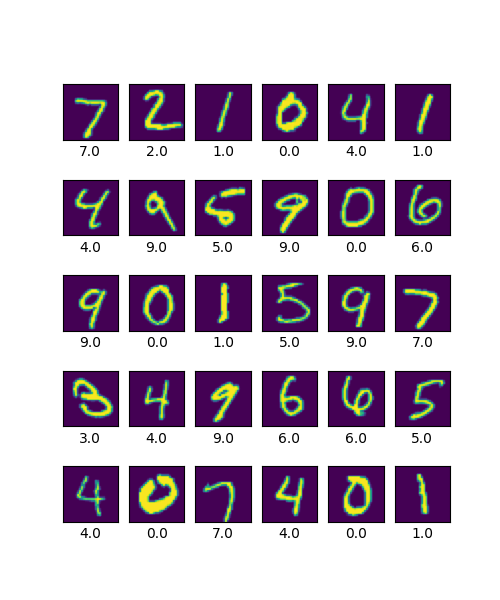
\includegraphics[width=\linewidth]{dataset_mnist.png}
    $ZT1$
\endminipage\hfill
\minipage{0.32\textwidth}
    \centering
    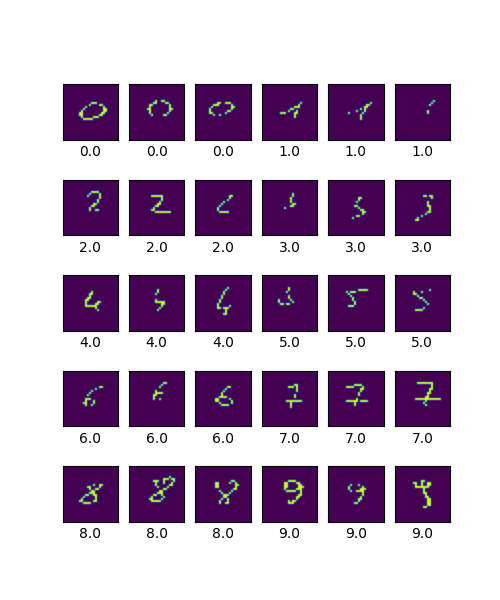
\includegraphics[width=\linewidth]{dataset_my.png}
    $ZT2$
\endminipage\hfill
\minipage{0.32\textwidth}
    \centering
    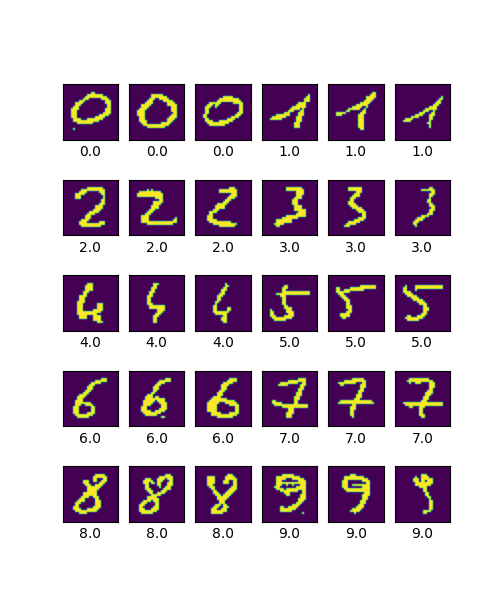
\includegraphics[width=\linewidth]{dataset_my_preprocessed.png}
    $ZT2\_PREPROCESSED$
\endminipage
\end{figure}

\section*{Wybór parametrów}
Początkowe parametry do wyboru struktury sieci to:
\begin{itemize}
    \item batch\_size = 8
    \item epochs = 10
    \item optimizer = adam
    \item loss = Sparse Categorical Crossentropy
\end{itemize}
Każda sieć przyjmuje input rozmiaru (28 x 28). Ostatnią warstwą zawsze jest $Dense$, która łączy sie z każdym elementem poprzedniej warstwy i tworzy wektor 10-elementowy na wyjściu (1 element odpowiada jednej kategorii). Poniżej będę testował warstwy ukryte po środku:\\

\renewcommand{\arraystretch}{1.5}
\newcolumntype{M}[1]{>{\centering}m{#1}}

\phantom{.}\\
\begin{tabular}{ |M{3cm}|M{2cm}|M{2cm}|M{2cm}|M{2cm}|M{2cm}|c| } 
    \hline
        Struktura wewnętrzna sieci & $ZT1$ & $ZT2$ & $ZT2\_PRE$ & $ZT3$ & $ZT3\_PRE$ & \\
    \hline
        \multirow{2}{3cm}{\centering Flatten() Dense(64)} & 0.114 & 4.506 & 2.872 & 4.021 & 4.158 & loss \\
        & 97\% & 27\% & 63\% & 27\% & 53\% & accuracy\\
    \hline
        \multirow{2}{3cm}{\centering Flatten() Dense(128)} & 0.101 & 6.919 & 3.429 & 7.162 & 4.882 & loss \\
        & 98\% & 27\% & 60\% & 17\% & 57\% & accuracy\\
    \hline
        \multirow{2}{3cm}{\centering Flatten() Dense(256)} & 0.126 & 6.971 & 4.221 & 6.654 & 5.564 & loss \\
        & 98\% & 27\% & 60\% & 23\% & 63\% & accuracy\\
    \hline
        \multirow{2}{3cm}{\centering Flatten() Dense(196) Dense(49)} & 0.096 & 6.387 & 4.806 & 4.954 & 2.724 & loss \\
        & 98\% & 23\% & 67\% & 30\% & 70\% & accuracy\\
    \hline
        \multirow{2}{3cm}{\centering Flatten() Dense(392) Dense(98) Dense(24)} & 0.122 & 4.364 & 2.442 & 4.223 & 2.817 & loss \\[8pt]
        & 98\% & 30\% & 53\% & 33\% & 67\% & accuracy \\[8pt]
    \hline
        \multirow{2}{3cm}{\centering Conv2D(32) MaxPool2D() Flatten()} & 0.061 & 5.642 & 3.361 & 5.955 & 3.196 & loss \\
        & 99\% & 27\% & 67\% & 23\% & 63\% & accuracy \\
    \hline
        \multirow{2}{3cm}{\centering Conv2D(32) MaxPool2D() Conv2D(32) MaxPool2D() Flatten()} & 0.051 & 8.359 & 1.831 & 8.374 & 2.769 & loss \\[12pt]
        & 99\% & 13\% & 80\% & 30\% & 63\% & accuracy \\[12pt]
    \hline
        \multirow{2}{3cm}{\centering Conv2D(32) MaxPool2D() Conv2D(32) MaxPool2D() Conv2D(32) MaxPool2D() Flatten()} & 0.079 & 6.099 & 1.682 & 5.271 & 2.703 & loss \\[24pt]
        & 99\% & 30\% & 80\% & 40\% & 70\% & accuracy \\[24pt]
    \hline
    %     \multirow{2}{3cm}{\centering } &  &  &  &  &  & loss \\[8pt]
    %     & \% & \% & \% & \% & \% & accuracy \\[8pt]
    % \hline

\end{tabular}

\phantom{.}\\
Najbardziej optymalne wyniki zwraca sieć złożona z trzech zestawów (Conv2D + MaxPool2D).

\section*{Wnioski}
Dla danych ze zbioru MNIST, które są identycznie przygotowane jak dane na których sieć była uczona, w stosunkowo krótkim czasie da się osiągnąć wskaźnik prawidłowej rozpoznawalności powyżej 99\%.\\
Dla danych stworzonych przez osoby trzecie, bardzo ważne jest jak najdokładniejsze przygotowanie tych danych. Przy minimalnym przygotowaniu ($ZT2$ i $ZT3$) sieć wskazuje poprawne wyniki w około $30\% \pm 3\%$. Natomiast dane preprocesowane podobnie do danych MNIST ($ZT2\_PREPROCESSED$ i $ZT3\_PREPROCESSED$) potrafiły uzyskać około $65\% \pm 10\%$.

\end{document}

